\chapter{Evaluation}
As mentioned in the methodology, the evaluation was carried out during all the development lifecycle allowing improvements with respect to each iteration. This chapter describes how the evaluation of a final prototype was carried out to assess functional and non functional aspects, as well as the technical evaluations that were performed during the development to ensure the accomplishment of the software quality attributes. 

\section{Technical Evaluation}

\subsection{Automated tests}

Testing an Android application is particularly challenging because as opposed with iOS, many manufacturers are allowed to distribute their own devices that run this operative system. This means that an application should be able to work in many different phones with different screen sizes, resolutions or specific hardware components. There is not a proven way to test an android application other than trying it out on many distinct devices. This normally is an expensive task, but nowadays emerging services make available cloud based devices so that developers can connect to them remotely to install and test their applications on demand.

Amazon provides such service in the AWS mobile device farm \footnote{\url{https://aws.amazon.com/device-farm/}}. The application was tested by executing automated tests that explore the interface autonomously to discover how it might react to normal user interaction but also under odd circumstances. Another benefit of this service is that the tests are executed in parallel with a number of devices that are widely used (in this case 15) to encounter errors that might arise from different screen types or hardware components. 

The test starts by uploading a packaged version of the application to the service who is responsible to install it in different devices of the farm. If the application is able to respond to all simulated user input and keep working under a defined period of time then the test for that specific device is passed. Two iterations of this test allowed to find bugs and interface errors that were corrected and optimized. In the first test carried out the application was failing on 5 from 15 devices, the logs of the crash were studied and fixed. A second iteration showed a better outcome, just 1 of the 15 devices were failing the test. Resulting in an improved compatibility.   

\begin{figure}[H]
\begin{adjustbox}{width=1\textwidth,center=\textwidth}
  \centering
  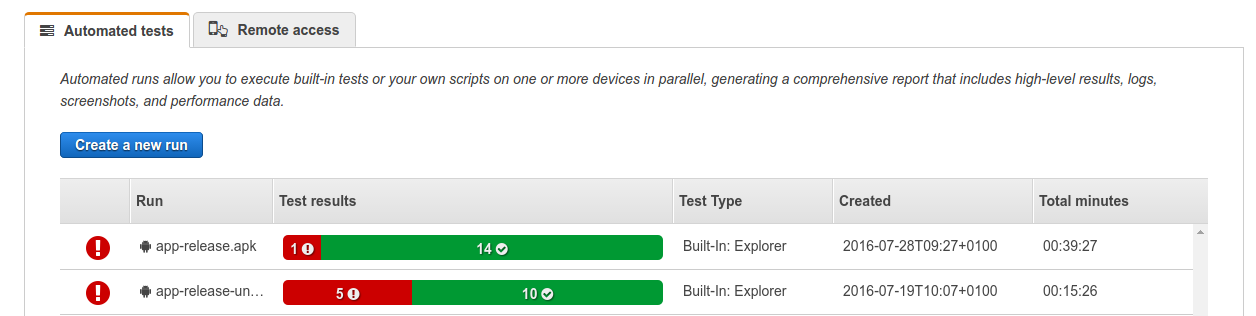
\includegraphics[scale=1]{images/automated_tests.png}
\end{adjustbox}
  \caption[Automated tests on AWS]{Automated tests on AWS}
  \label{fig:automated_tests}
\end{figure}

\subsection{Resource usage}
In order to ensure that the application consumes the adequate number of resources from any device, it is straightforward to inspect the resource usage of the running application. Android provides tools to monitor the usage of the consumed resources such as battery, bandwidth and memory from any application installed. From its usage the following was identified:
\begin{itemize}
	\item Memory: The application consumes in total 33mb in storage, which is not extraordinary compact but is feasible given the modern phones storage capabilities. 
    \item Data usage: For all the development process the application was executed several times during almost a month. It used 2.15mb of data in total. Which is a very good performance for an application of this kind.
    \item Battery usage: From using the application on repeated occasions in a dedicated device, it was found that the application doesn't reach the list of top battery consumer services in the phone. The reason for this is that the it doesn't employ any background process, all the communication tasks are performed when the app is open. Also, it does not require the GPS to be on as it will use the location already gathered by the internal phone services.
\end{itemize}


\begin{figure}[H]
\begin{adjustbox}{width=.45\textwidth,center=\textwidth}
  \centering
  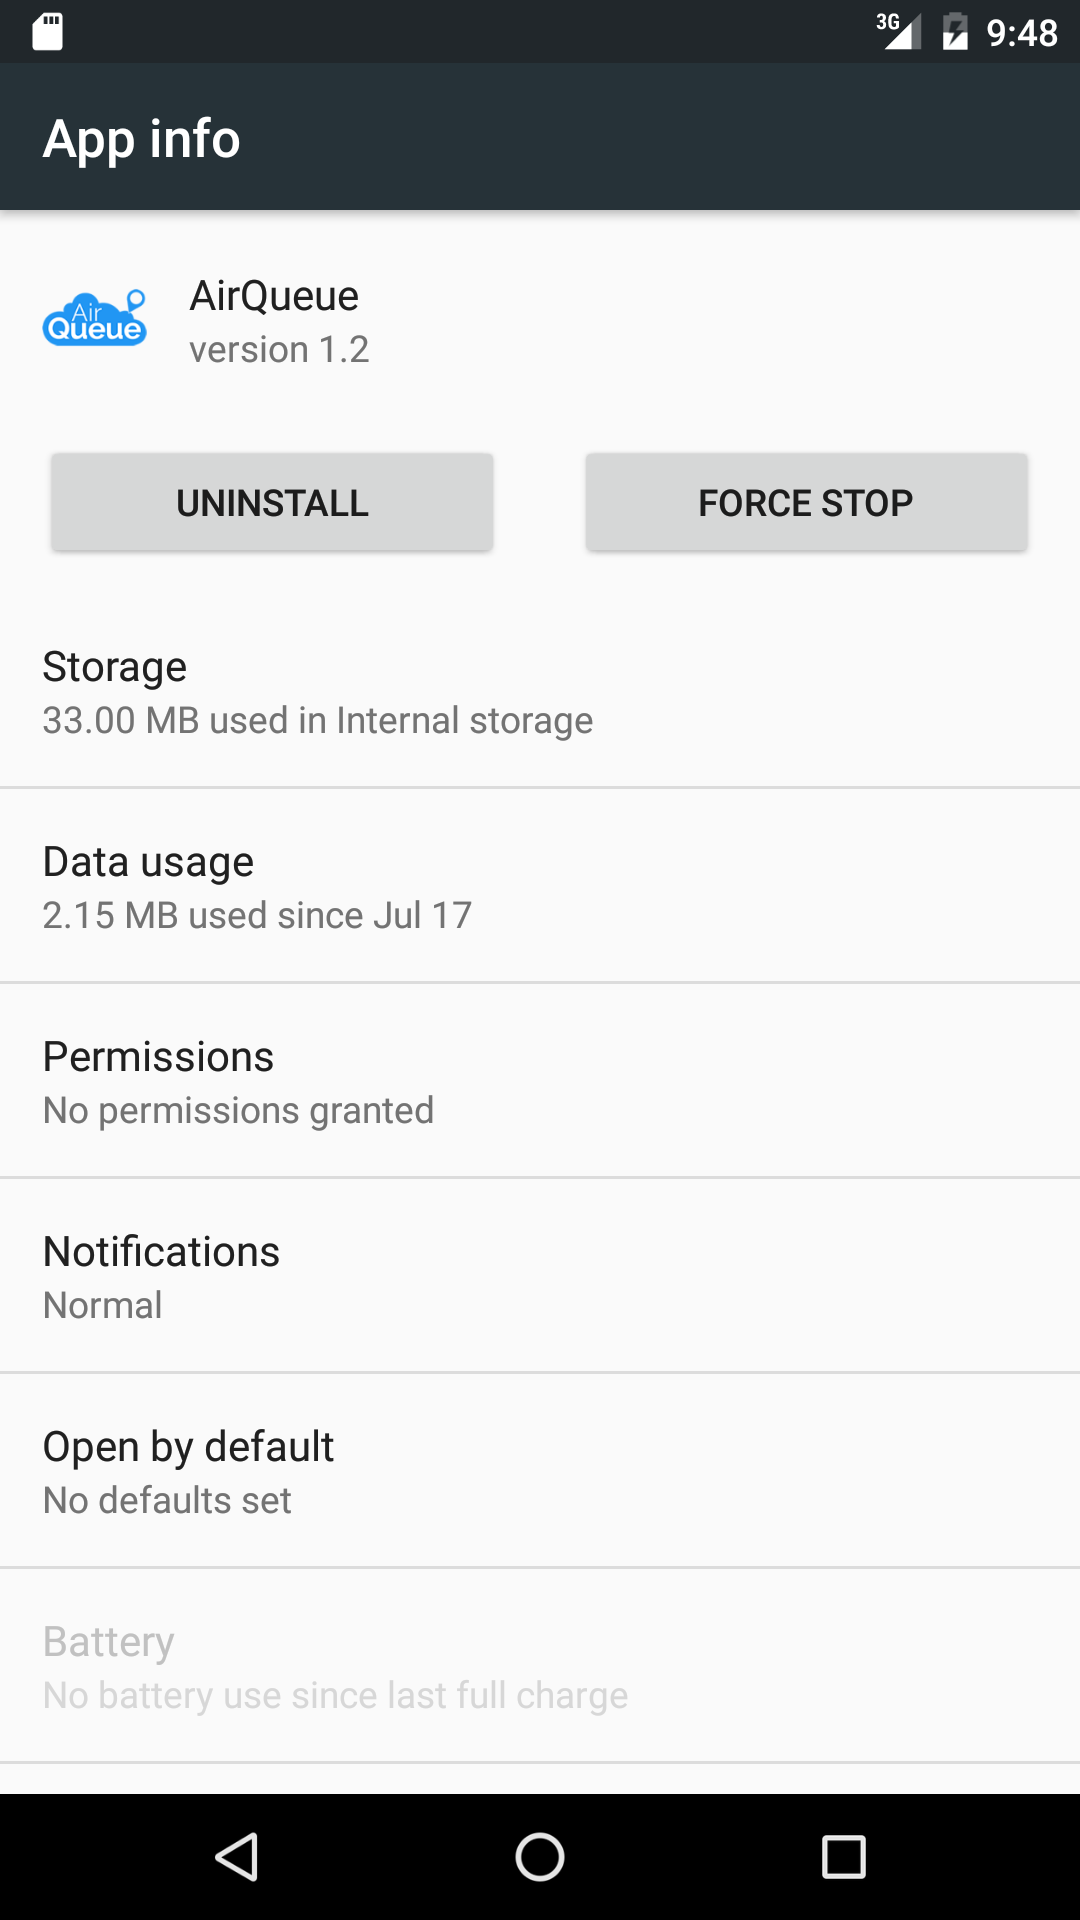
\includegraphics[scale=1]{images/resource_usage.png}
\end{adjustbox}
  \caption[Application resource usage]{Application resource usage}
  \label{fig:automated_tests}
\end{figure}


\section{Evaluation with users}

The evaluation of a third prototype was carried out with potential final users of the application. That is, with volunteers from the AUKAR group, and from general users from the University of Edinburgh. Two methods were employed for this purpose, a usability test complemented by a design critique. 

\subsection{Usability testing}
To ensure that the functional requirements as well as the usability attributes are accomplished, it is helpful to test the product with real users under real world circumstances. This would outcome on getting a more accurate feedback on how well users are interacting with the product in terms of the remaining selected attributes: usability and performance.

In total there were three participants, one from AUKAR, and two from the University of Edinburgh. All of them were new to the application. For the set-up, an android phone (Motorola Moto G 3rd Gen.) was configured with the AirQueue app and a screen logger. The room was equipped with a video recorder to keep log of the said by the participants. The test was divided in two parts in a one hour individual meeting. 

The first part of the test consisted in executing small tasks or scenarios that should be accomplished within the interface, covering tasks in all visualizations and screens. Participants were asked to perform them individually and to indicate if they were able to do so with ease. Also, some of them were thinking aloud during the test. 

P1, P2 and P3 are the participants of the test. Their ages were 68, 28 and 27 respectively. Their occupations are retired, designer and biologist. Each participant marked whether they were able to finish each of the tasks with ease as instructed with n (No) or y (yes). The findings and the scenarios are shown in Table \ref{tab:test_scenarios}.

In general the users were able to follow up the instructions one by one using the visual and textual cues provided. From the screen video logging was found that users were trying to interact with the elements of the screen to discover their usage (even if some components were not providing any usage), also, the tool-tips served a good guiding function, all the participants used them to understand better the navigation through the interface. The screen with the better success rate was (PEND). 

\begin{figure}[H]
\begin{adjustbox}{width=.8\textwidth,center=\textwidth}
  \centering
  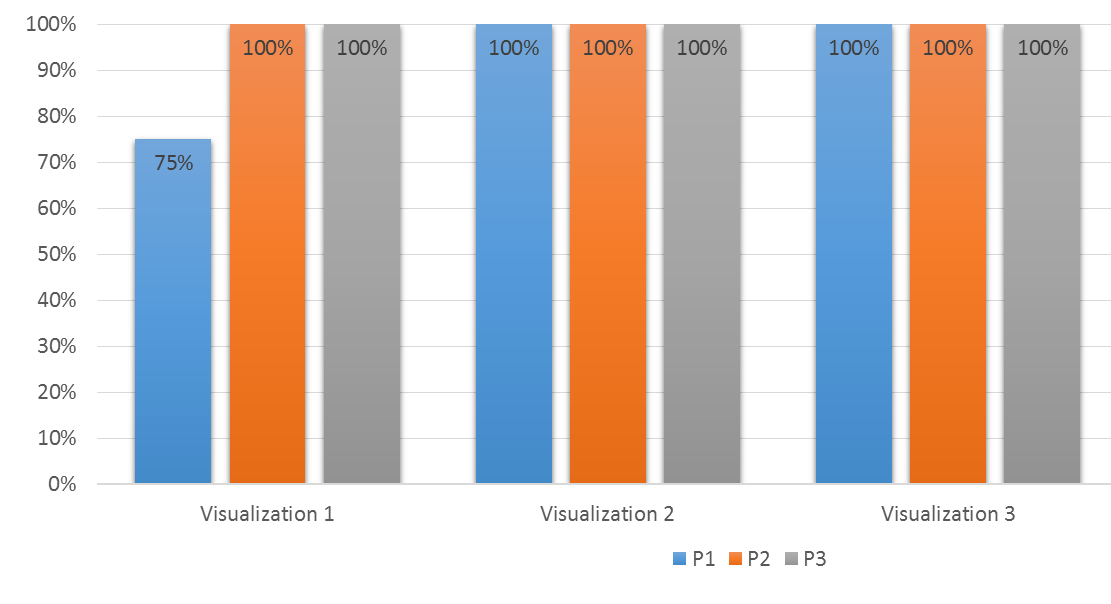
\includegraphics[scale=1]{images/scenarios_rate.png}
\end{adjustbox}
  \caption[Scenario tests completion rate]{Scenario tests completion rate}
  \label{fig:automated_tests}
\end{figure}

\newcommand{\specialcell}[2][c]{%
  \begin{tabular}[#1]{@{}l@{}}#2\end{tabular}}

\begin{table}[H]
\centering
\begin{adjustbox}{width=1\textwidth,center=\textwidth}
\begin{tabular}{llrrr}
  \hline
   Tab/Screen & Activity & P1 & P2 & P3 \\ \hline
   Overview & \specialcell[t]{1.-I want to start the application and reach the first\\'overview' screen.}  & y & y & y \\
   Overview & \specialcell[t]{2.-I want to visualize the location of the closest air\\quality-sensor and know when was it last updated. (Just\\read the information).} & y & y & y \\
   Overview & \specialcell[t]{3.-I want to adjust my sensitivity level to indicate I have\\high sensitivity.} & y & y & y \\
   Overview & \specialcell[t]{4.-I want to know the air quality index. (How good or bad\\the air quality is).} & y & y & y \\
   Overview & \specialcell[t]{5.-I want to read my personalized health advice. (Just\\read the information)} & y & y & y \\
   Overview &\specialcell[t]{6.-I want to adjust again my sensitivity level to indicate I\\have a low sensitivity and read my advice again.} & y & y & y \\
   Pollutants &\specialcell[t]{7.-I want to navigate to the second 'Pollutants' screen.} & y & y & y \\
   Pollutants &\specialcell[t]{8.-I want to examine the measured value for the sulphur\\dioxide pollutant.} & n & y & y \\
   Pollutants &\specialcell[t]{9.-I want to know if the measured value for sulphur\\dioxide is categorized as good, regular, bad or extremely\\bad.} & y & y & y \\
   Pollutants &\specialcell[t]{10.-I want to know further information about particulate\\matter. I want to read the sources and health effects of\\
   this specific pollutant.} & y & y & y \\
   Graphs &\specialcell[t]{11.-I want to navigate to the third 'Graphs' screen.} & y & y & y \\
   Graphs &\specialcell[t]{13.-I want to select the 'CO' pollutant and visualize the\\measured values through the day.} & y & y & y \\
   Graphs &\specialcell[t]{14.-I want to select the PM10 pollutant and visualize the\\measured values for yesterday.} & y & y & y \\
   \hline
\end{tabular}
\end{adjustbox}
  \caption[Usability testing scenarios]{Usability testing scenarios and results}
\label{tab:test_scenarios}
\end{table} 

The second part of the usability test was guided by an usability scale. The users were asked to evaluate their experience ranking their agreement over different statements. Where 1 was strongly disagree and 5 was strongly agree. The employed usability scale and the responses are shown in Table \ref{tab:test_usability_scale}.

\begin{table}[H]
\centering
\begin{adjustbox}{width=1.2\textwidth,center=\textwidth}
\begin{tabular}{llrrr}
  \hline
   - & Statement & P1 & P2 & P3 \\ \hline
   Overview & \specialcell[t]{1.-I think that the first screen (overview) was easy to\\understand/navigate.} & 3 & 1 & - \\
   Overview &\specialcell[t]{2.- I think that the 'overview' screen would help me to understand the\\current situation of air quality.} & 5 & - & - \\
   Overview &\specialcell[t]{3.- I think that the personalized health 'advice' would help me to take better\\choices through the day.} & 5 & - & - \\
   Overview &\specialcell[t]{4.- I feel that is useful to know the location of the closest air quality sensor.} & 5 & - & - \\
   Overview &\specialcell[t]{5.- I think that the colours of the 'overview' screen help me to\\understand the usage of the screen components.} & 1 & - & - \\
   Overview &\specialcell[t]{6.- In the 'overview' screen, I think that the wording of the menus, labels and\\pop-ups is clear and concise.} & 3 & - & - \\
   Pollutants &\specialcell[t]{7.- I think that the second screen (pollutants) was easy to\\understand/navigate.} & 5 & - & - \\
   Pollutants &\specialcell[t]{8.- The 'pollutants' screen would help me to understand the current situation of air\\quality.} & 5 & - & - \\   
   Pollutants &\specialcell[t]{9.- In the 'pollutants' screen the individual pollutant circles help me to understand\\easily how good or bad the measurements are. } & 5 & - & - \\   
   Pollutants &\specialcell[t]{10.- It is useful to have information about the sources and effects of air pollution. } & 5 & - & - \\   
   Graphs &\specialcell[t]{11.- I think that the third screen (graphs) was easy to understand/navigate.} & 5 & - & - \\   
   Graphs &\specialcell[t]{12.- I think that the third screen 'Graphs' would be useful to track my response to\\certain pollutants.} & 5 & - & - \\   
   Graphs &\specialcell[t]{13.- In the graphs screen the pollutant different colours help me to differentiate them.} & 5 & - & - \\   
   Graphs &\specialcell[t]{14.- In the third screen (Graphs) the pollutant graphs are displayed promptly.} & 5 & - & - \\   
   App in general &\specialcell[t]{15.- I think that it was easy to access and navigate through all the three screens.} & 4 & - & - \\     
   App in general &\specialcell[t]{16.- I would imagine that most people would learn to use this system very quickly.} & 4 & - & - \\ 
   App in general &\specialcell[t]{17.- I needed to learn a lot of things before I could get going with this system.} & 5 & - & - \\ 
   App in general &\specialcell[t]{18.- I would say that the colours of the application help me to understand it better.} & 5 & - & - \\ 
   App in general &\specialcell[t]{19.- I think that the application response to my actions wast fast and smooth.} & 5 & - & - \\    
   App in general &\specialcell[t]{20.- The application starts promptly } & 5 & - & - \\       
   App in general &\specialcell[t]{21.- I thought that simple indicators such as 'good', 'regular', 'bad' helped to understand\\the current air quality status.} & 5 & - & - \\       
   App in general &\specialcell[t]{22.- I thought that colour indicators (green/yellow/red) helped to understand the\\current air quality status.} & 5 & - & - \\          
   App in general &\specialcell[t]{23.- I would use this application to make better choices about my health.} & 5 & - & - \\             
   App in general &\specialcell[t]{24.- I would use this application to know more about pollution in general.} & 5 & - & - \\                
   App in general &\specialcell[t]{25.- I think using this application is fun and enjoyable.} & 3 & - & - \\         
   App in general &\specialcell[t]{26.- Having an 'smart' health advice   would help making my life easier.} & 5 & - & - \\      
   App in general &\specialcell[t]{27.- It is more engaging or interesting using an application instead of a website to get\\information about pollution} & 5 & - & - \\         
   \hline
\end{tabular}
\end{adjustbox}
  \caption[Usability testing scenarios]{Usability testing scenarios and results}
\label{tab:test_usability_scale}
\end{table} 

\subsection{Design critique}
At the end of the meeting, participants were asked to give their thoughts on the application. This was an open discussion where the participants where guided through a couple of questions to find out more about what did they like, dislike, find useful or would add to the application. 

\bigskip
\textbf{What do you think about the interface?}
\bigskip

\begin{itemize}
	\item "The interface is very clean."
    \item "It looks nice."
    \item "This is almost like the front page on a book isn't it?" - Referring to the first screen.
    \item "I didn't realize how to move away this tool-tip."
\end{itemize}

\bigskip
\textbf{Do you think having an application like this would help you to stay more informed about air pollution?}
\bigskip

\begin{itemize}
	\item "It would, because that way I can decide what to do based on what I see."
	\item "Certainly It would be a great help."
\end{itemize}

\bigskip
\textbf{If you could add something, what would it be?}
\bigskip

\begin{itemize}
	\item "I was expecting this to react, it didn't occur to me that it was an introduction."
    \item "Maybe the ability to select other sensors from this screen."
\end{itemize}

\bigskip
\textbf{What do you like about the application?}
\bigskip

\begin{itemize}
	\item "I like the way you can adjust, presumably once you've adjust it, everything else in the screen takes it into account."
\end{itemize}

